The simplest way of approaching the evolutionary search problem for test case generation is by iteratively determining a coverage goal in the source code (i.e. a particular branch), and executing the GA to find a test case that achieves this coverage. 
A strategy for iterative search typically includes:
\begin{itemize}
    \item Enumerating the targets to cover, i.e. the individual branches.
    \item Performing the single-objective search for each target, until all the targets are covered, or the budget has expired.
    \item Building the final test suite by combining 
\end{itemize}



Focusing on one coverage goal at a time is ultimately a poor strategy, however, since it assumes that all coverage goal are equally important and independent of each other; this is often not the case as, for example, covering the true branch of an if statement may be easier than covering the true branch of another if statement that requires a complex chain of operations to be properly satisfied. A search algorithms could get "trapped" while attempting to cover an expensive branch and waste a large portion of the testing budget.

Additionally, covering a particular branch may have collateral coverage over other branches in the test case's path; this suggests that multi-target approaches may reveal more effective. These approaches are known as whole test suites approaches and their goal is to evolve the entire test suite simultaneously, rather than iteratively covering the single branches/statements.


------------------------------------------------------------------------------------------
Specifically, the fitness function is mainly based on two measures:
approach level and branch distance. The approach level represents how
far is the execution path of a given test case from covering the target branch,
while the branch distance represents how far is the input data from changing the
boolean value of the condition of the decision node nearest to the target branch.
As the branch distance value could be arbitrarily greater than the approach
level, it is common to normalize the value of the branch distance.
------------------------------------------------------------------------------------------

EvoSuite is an example of an evolutionary algorithm that optimizes the whole test suite towards just one coverage criterion, rather than generating test cases directed towards multiple coverage criteria.
With EvoSuite, any collateral coverage isn't a concern since all coverage is intentional, given that the ultimate goal is to generate the whole test suite.
The algorithm starts with a randomly generated population of test suites.
The fitness function rewards better coverage of the source code; if two suites have the same coverage, the one with fewer statements is chosen. For each test suite, its fitness is measured by executing all of its test cases and keeping track of the executed methods and of the minimal branch distance for each branch.

\textbf{Expand on bloat in EvoSuite}


Another popular algorithm for multi-target search problems is the Non-dominated Sorting Genetic Algorithm II (NSGA-II). This algorithm is based on three principles:

\begin{itemize}
    \item It uses elitism when evolving the population: the most fit individuals are carried over along the offsprings.
    \item It uses an explicit diversity-preserving mechanism, the Crowding distance.
    \item It emphasizes the non-dominated solutions, as its name suggests.
\end{itemize}

First of all, in the context of test cases, domination can be expressed by the following relation:
\begin{figure}[!h]
    \centering
    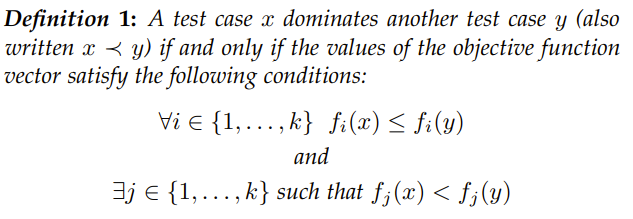
\includegraphics[scale=0.4]{./figures/test_Case_domination.PNG}
    \caption{Test case domination}
    \label{fig:test case domination}
\end{figure}


The NSGA-II algorithm works as follows:
\begin{itemize}
    \item Starting from an initial population of individuals Pt, generate an offspring population Qt of equal size and merge the two together, obtaining the population Rt.
    \item Perform non-dominated sorting of the individuals in Rt based on target indicators and classify them by fronts, i.e. they are sorted according to an ascending level of non-domination.  This ensures that the top Pareto-optimal individuals will survive to the next generation.
    \item If one of the fronts in the sorted sequence doesn't fit in terms of population size, crowding distance sorting is performed.
    \item Create the new population based on crowded tournament selection, then perform crossover and mutation. 
\end{itemize}


Figure 2.2 summarizes the main loop of the algorithm:
\begin{figure}[!h]
    \centering
    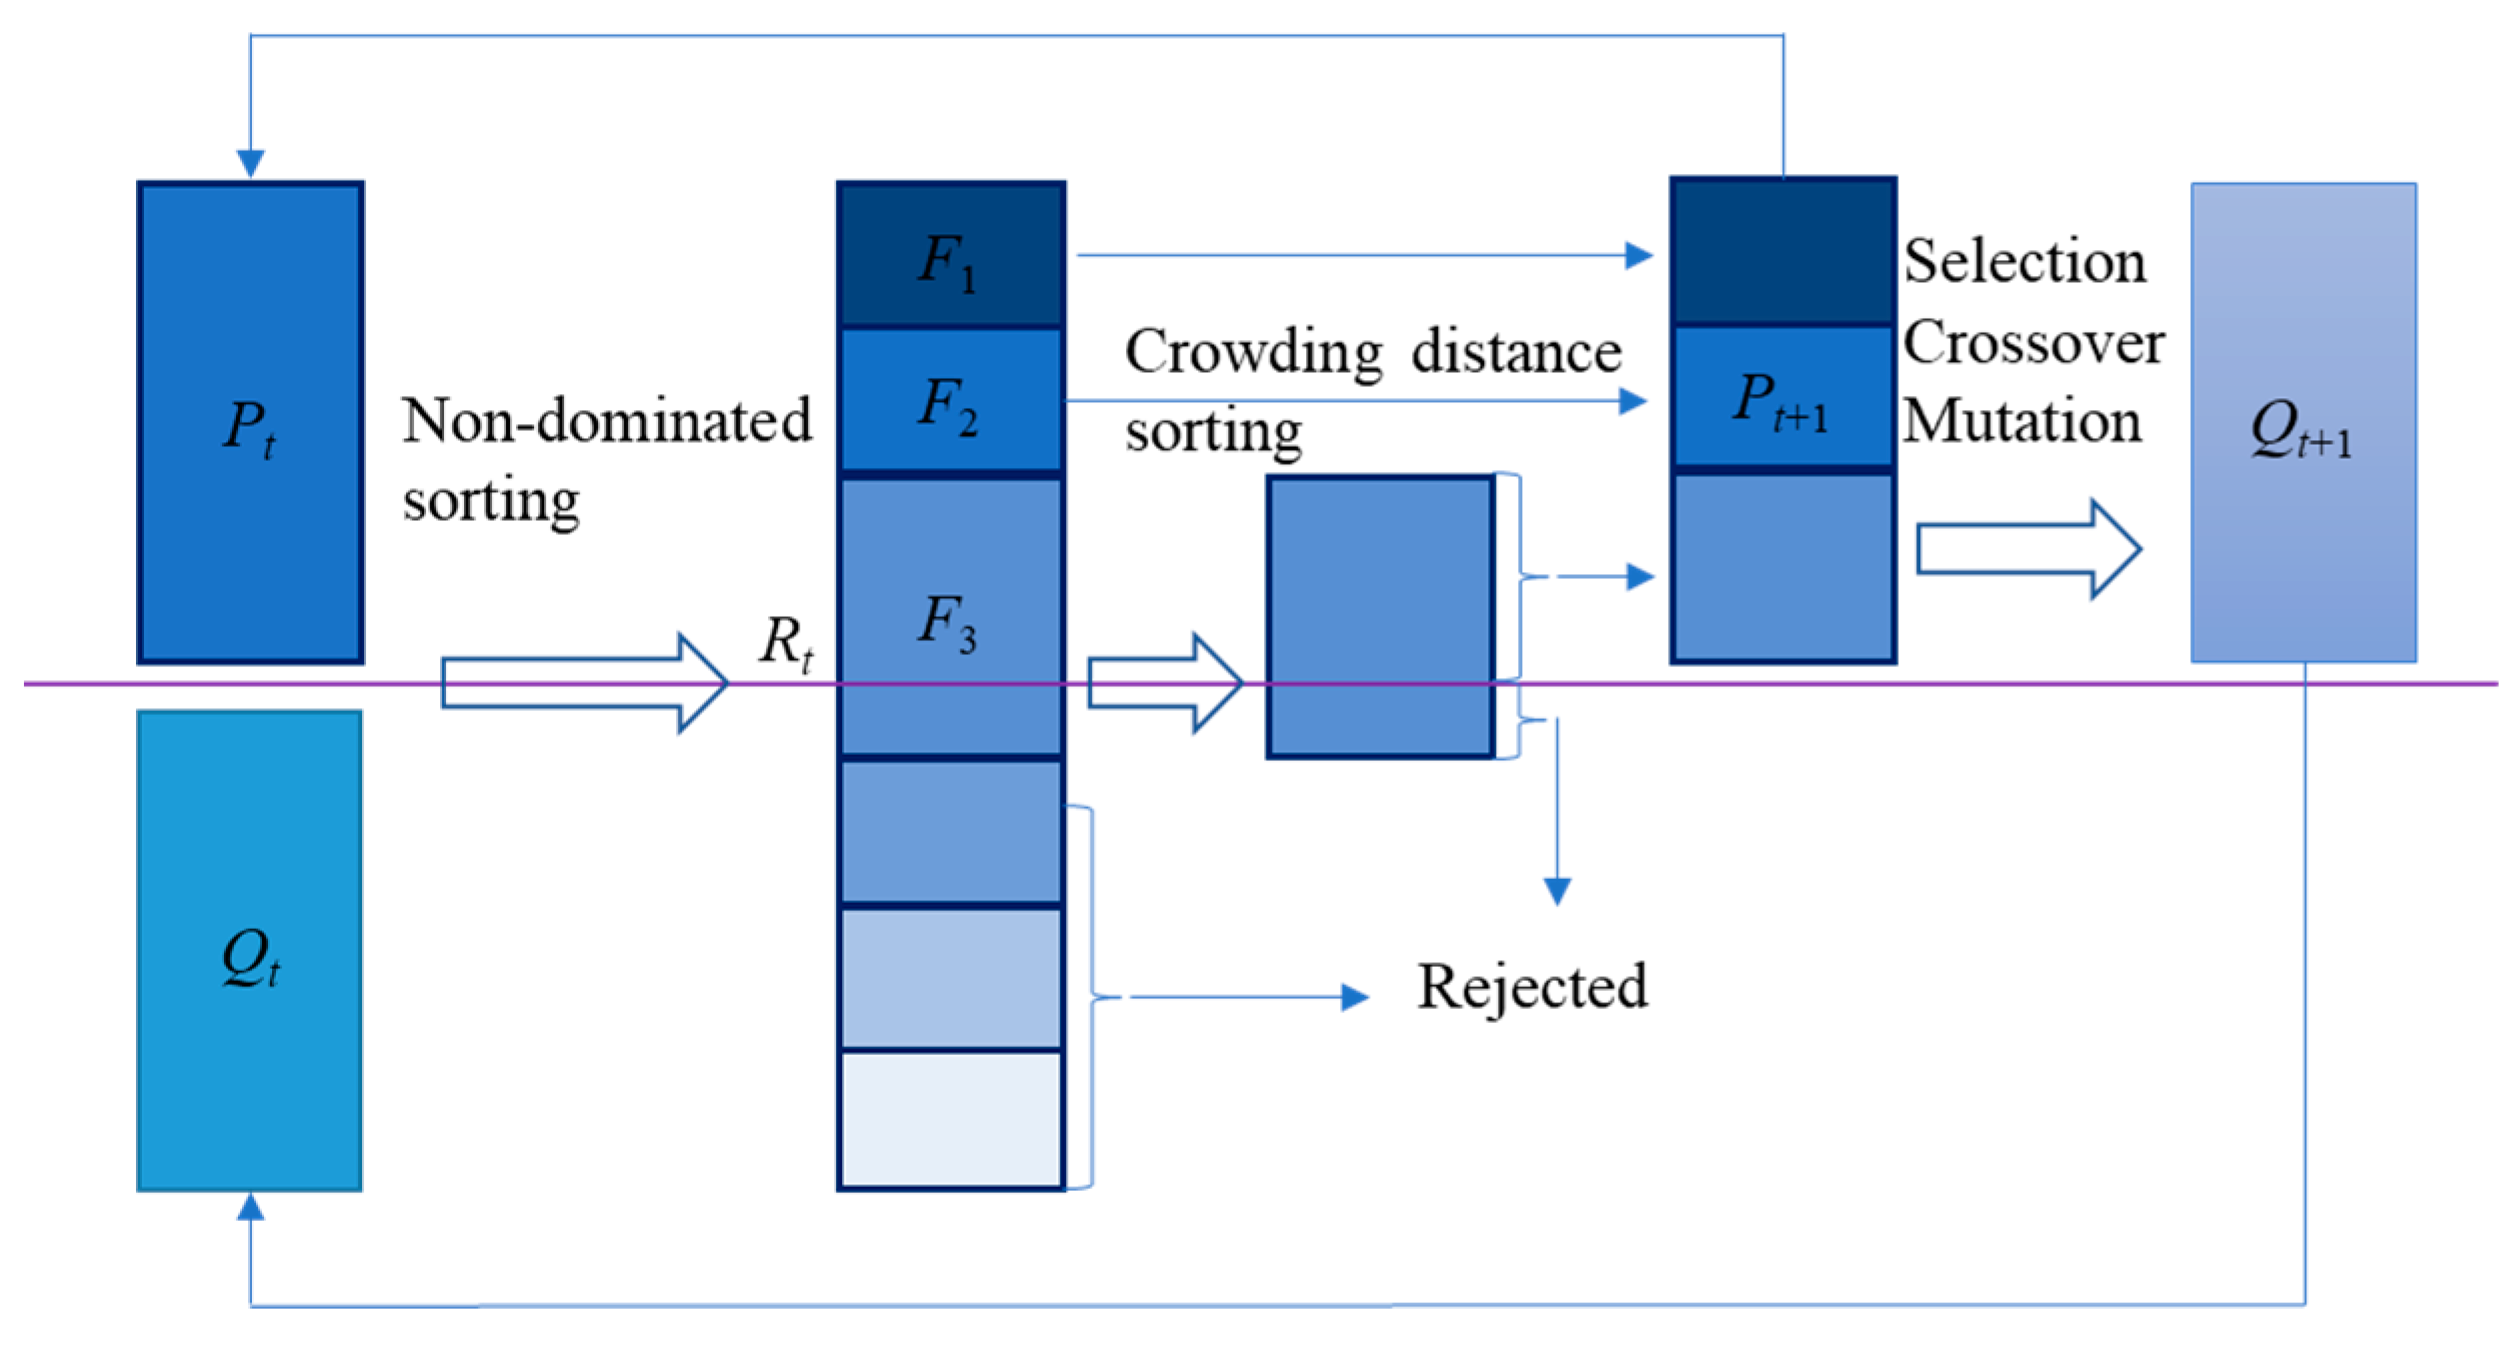
\includegraphics[scale=0.1]{./figures/nsga-ii.png}
    \caption{NSGA-II algorithm main loop}
    \label{fig:NSGA-II algorithm main loop}
\end{figure}


In the context of software engineering, NSGA-II has been applied to problems such as software refactoring and test case prioritization,
with two or three objectives. If the number of objectives begins to grow, however, the performance of the algorithm doesn't scale up well \cite{DBLP:journals/csur/LiLTY15}.
To overcome these limitation,


MOSA...

DynaMOSA, Dynamic Many-Objective Sorting Algorithm \cite{article1} is an approach that focuses on ..., and has been developed as an evolution of MOSA. This latter solution implements a many-objective GA to tackle test case generation and has three main features: 
\begin{itemize}
    \item instead of ranking candidates for selection based on their Pareto optimality, it uses a preference criterion. This criterion selects the test case with the lowest objective score for each uncovered target; these selected individuals are given a higher chance of survival, while other test cases are ranked with the traditional NSGA-II approach.
    \item The search is focused only on the uncovered coverage targets.
    \item All tests that satisfy one or more of the uncovered targets will be archived and used as the final test suite once the search ends.
\end{itemize}

In many-objective optimization problems, candidate solutions are typically evaluated in terms of Pareto dominance and Pareto optimality.

DynaMOSA has been employed with Java classes.



Optimal Coverage sEarch-based tooL for sOftware Testing, OCELOT \cite{DBLP:conf/ssbse/ScalabrinoGNOL16} is a test case generation tool for C programs that implements both a multi-target approach based on MOSA, and new iterative single-target appproach named LIPS, Linear Independent Path-based Search.